Máte žebřík dlouhý 10 metrů, který se opírá o zeď.
Vršek žebříku je 6 metrů vysoko a vršek padá rychlostí 2 metry za sekundu.
Jak rychle se v tomto okamžiku pohybuje spodek žebříku?

\solution{
	\begin{enumerate}

		\item  \textbf{Napřed nakreslíme situaci} -- Obrázek~\ref{fig:cv11_zebrik}.
			\begin{figure}[H]
				\centering
				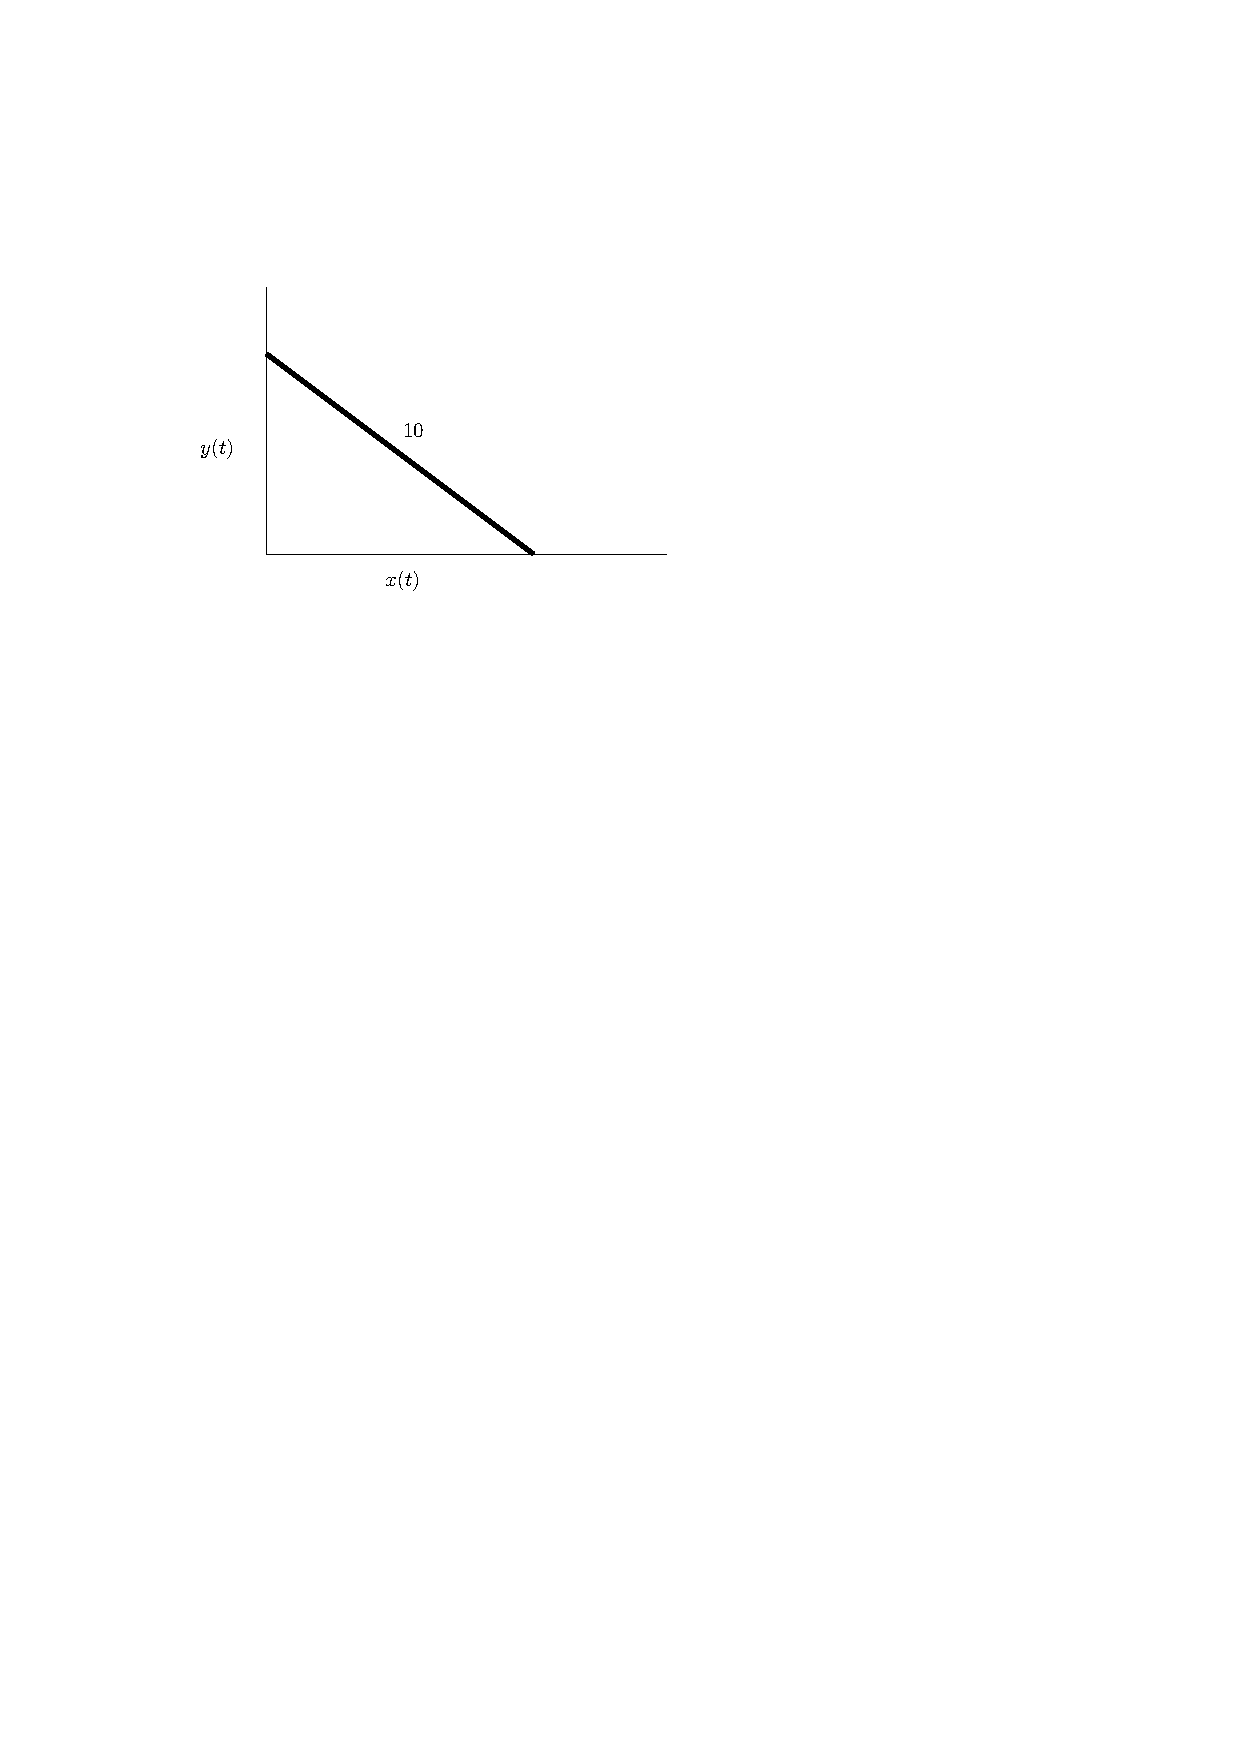
\includegraphics{cviceni_11/fig/zebrik.pdf}
				\caption{Obrázek žebříku, $y(t)$ je vzdálenost vršku žebříku od země v čase $t$, $x(t)$ je vzdálenost spodku žebříku od zdi v čase $t$.}
				\label{fig:cv11_zebrik}
			\end{figure}

		\item  \textbf{Co chceme určit?}
			Rychlost je derivace vzdálenosti podle času, fyzikálně zapsáno $dx/dt$.
			Tedy pokud $x(t)$ je naše vzdálenost od zdi v čase $t$, pak chceme první derivaci funkce $x$.

		\item  \textbf{Co známe? }

			\begin{itemize}

				\item  Známe derivaci výšky vršku žebříku $y'(t) = -2$ (žebřík padá, tedy $y(t)$ se zmenšuje).

				\item  Známe Pythagorovu větu: pro každý okamžik $t$ platí $x(t)^2 + y(t)^2 = 10^2$.

				\item  Tedy v tomto okamžiku platí $x(t)^2 + 6^2 = 10^2$, tedy $x(t) = 8$.

			\end{itemize}

		\item  \textbf{Zderivujeme obě strany Pythagorovy věty abychom dostali derivaci $x(t)$:}
			Obě strany jsou funkce času $t$ (pravá strana je konstantní funkce).
			Pokud jsou dvě funkce rovné, pak i jejich derivace by měly být rovné.
			\begin{align*}
				\left( x(t)^2 + y(t)^2 \right)' &= \left( 100^2 \right)' \\
				2x(t) x'(t) + 2y(t) y'(t) &= 0 \\
				x'(t) &= \frac{-2y(t) y'(t)}{2x(t)} \\
				x'(t) &= \frac{-2 \cdot 6 \cdot (-2)}{2 \cdot 8} \\
				x'(t) &= \frac{3}{2} \frac{m}{s}
			\end{align*}

		\item  \textbf{Odpovím:}
			Spodek žebříku se pohybuje rychlostí $3/2$ metru za sekundu směrem od zdi.

	\end{enumerate}
}

